\documentclass[12pt]{article} % use larger type; default would be 10pt
\usepackage[utf8]{inputenc} % set input encoding (not needed with XeLaTeX)

%%% PAGE DIMENSIONS
\usepackage{geometry} % to change the page dimensions
\geometry{a4paper} % or letterpaper (US) or a5paper or....
\geometry{margin=2cm} % or letterpaper (US) or a5paper or....

\usepackage{graphicx} % support the \includegraphics command and options
\usepackage[parfill]{parskip} % Activate to begin paragraphs with an empty line rather than an indent
\usepackage{times} % for Times Roman default font

%%% PACKAGES
\usepackage{booktabs} % for much better looking tables
\usepackage{array} % for better arrays (eg matrices) in maths
\usepackage{paralist} % very flexible & customisable lists (eg. enumerate/itemize, etc.)
\usepackage{verbatim} % adds environment for commenting out blocks of text & for better verbatim
\usepackage{subfig} % make it possible to include more than one captioned figure/table in a single float
\usepackage{hyperref} % make it possible to insert hyperlinks

%%% HEADERS & FOOTERS
\usepackage{fancyhdr} % This should be set AFTER setting up the page geometry
\pagestyle{fancy} % options: empty , plain , fancy
\renewcommand{\headrulewidth}{0pt} % customise the layout...
\lhead{}\chead{}\rhead{}
\lfoot{}\cfoot{\thepage}\rfoot{}

\makeatletter
\renewcommand{\maketitle}{%
  \begin{center}
    {\bfseries{\scshape{\Large{\@title\par}}}}
  \end{center}
  \medskip
  \begin{flushright}
    {\@date\par}
  \end{flushright}
    \bigskip\hrule\vspace*{2pc}%
}
\makeatother

\hyphenation{Kiwi-bank} % otherwise it may get hyphenated as Ki-wibank

%%% END Article customizations

%%% The "real" document content comes below...

\title{Springs Junction \href{https://www.warmshowers.org/}{WarmShowers} Information}
%\author{}
\date{\today} % Activate to display a given date or no date (if empty),
         % otherwise the current date is printed 

\begin{document}
  \maketitle

\begin{figure}[t]
%\centering
\begin{minipage}{.3\linewidth}
\begin{flushleft} 
   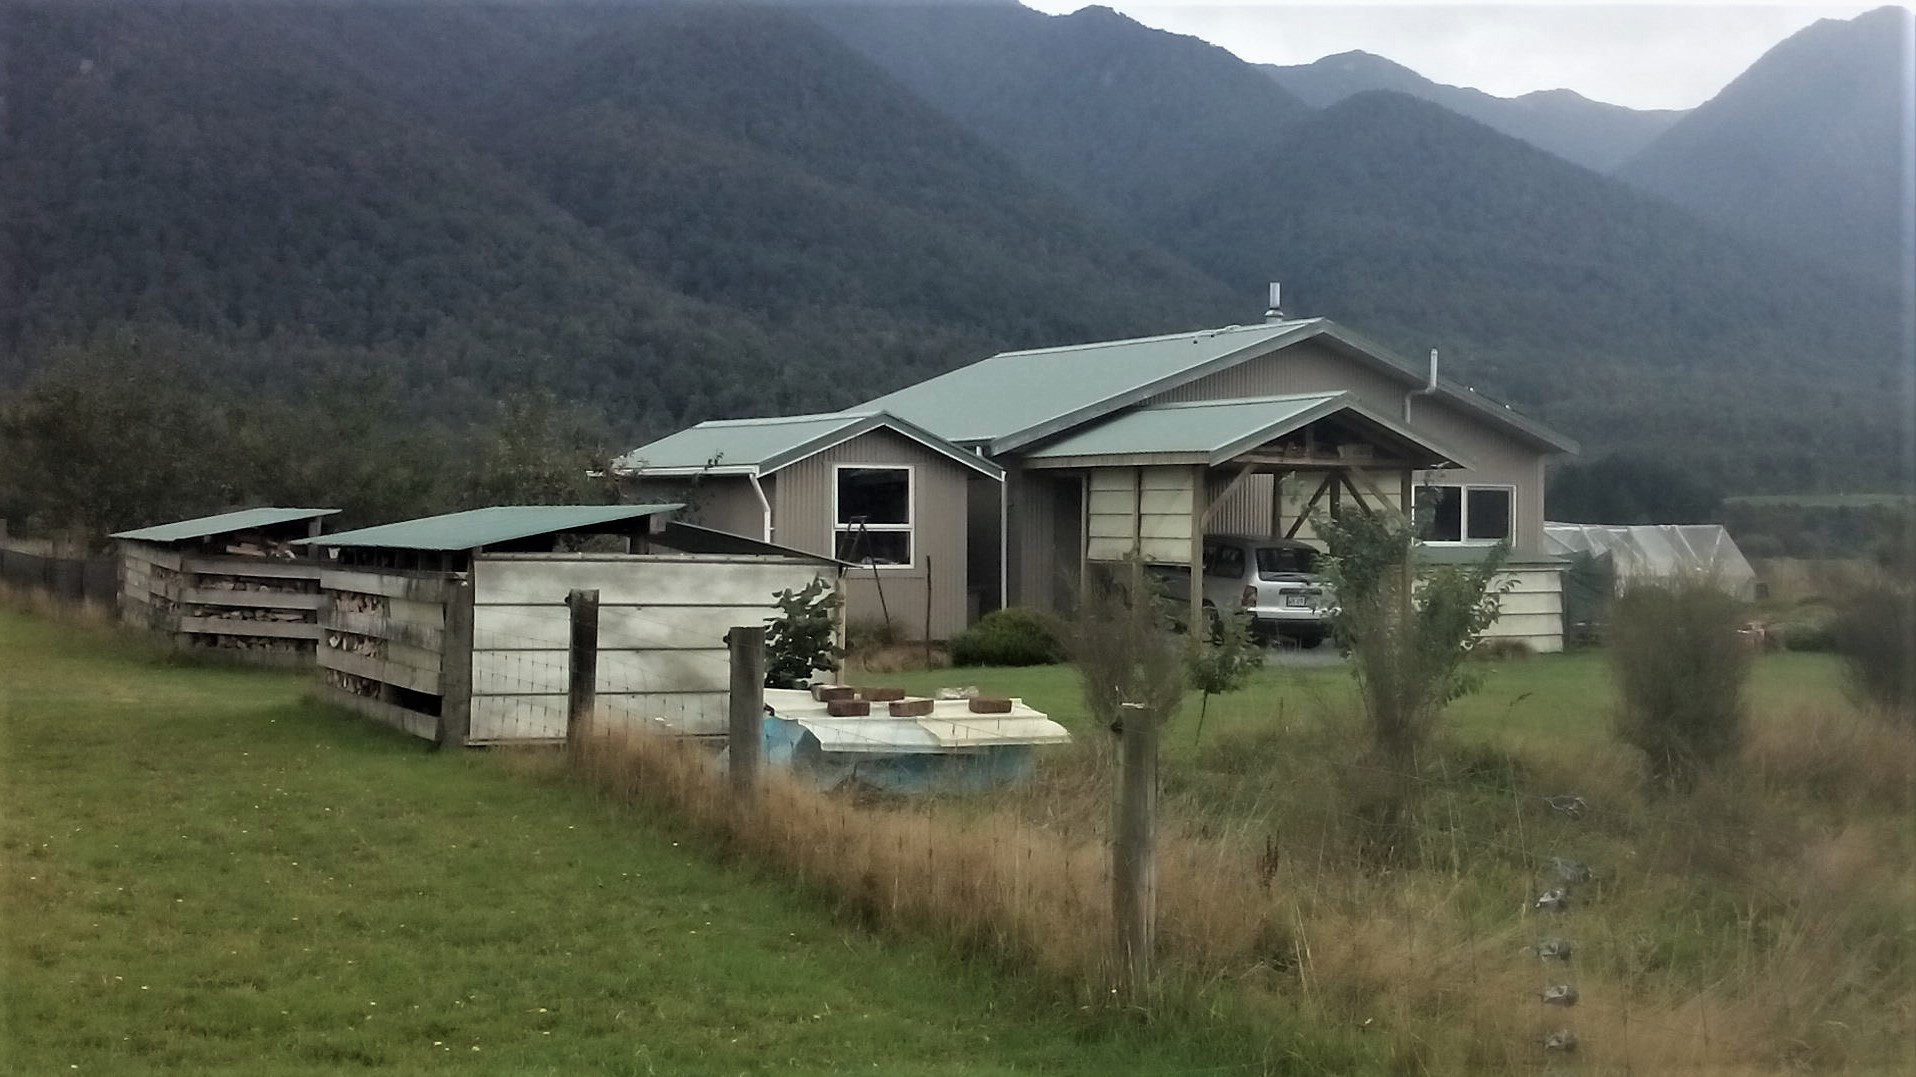
\includegraphics[width=4.5cm]{BachPhoto}
\end{flushleft} 
\end{minipage}
\begin{minipage}{.3\linewidth}
\begin{center} 
   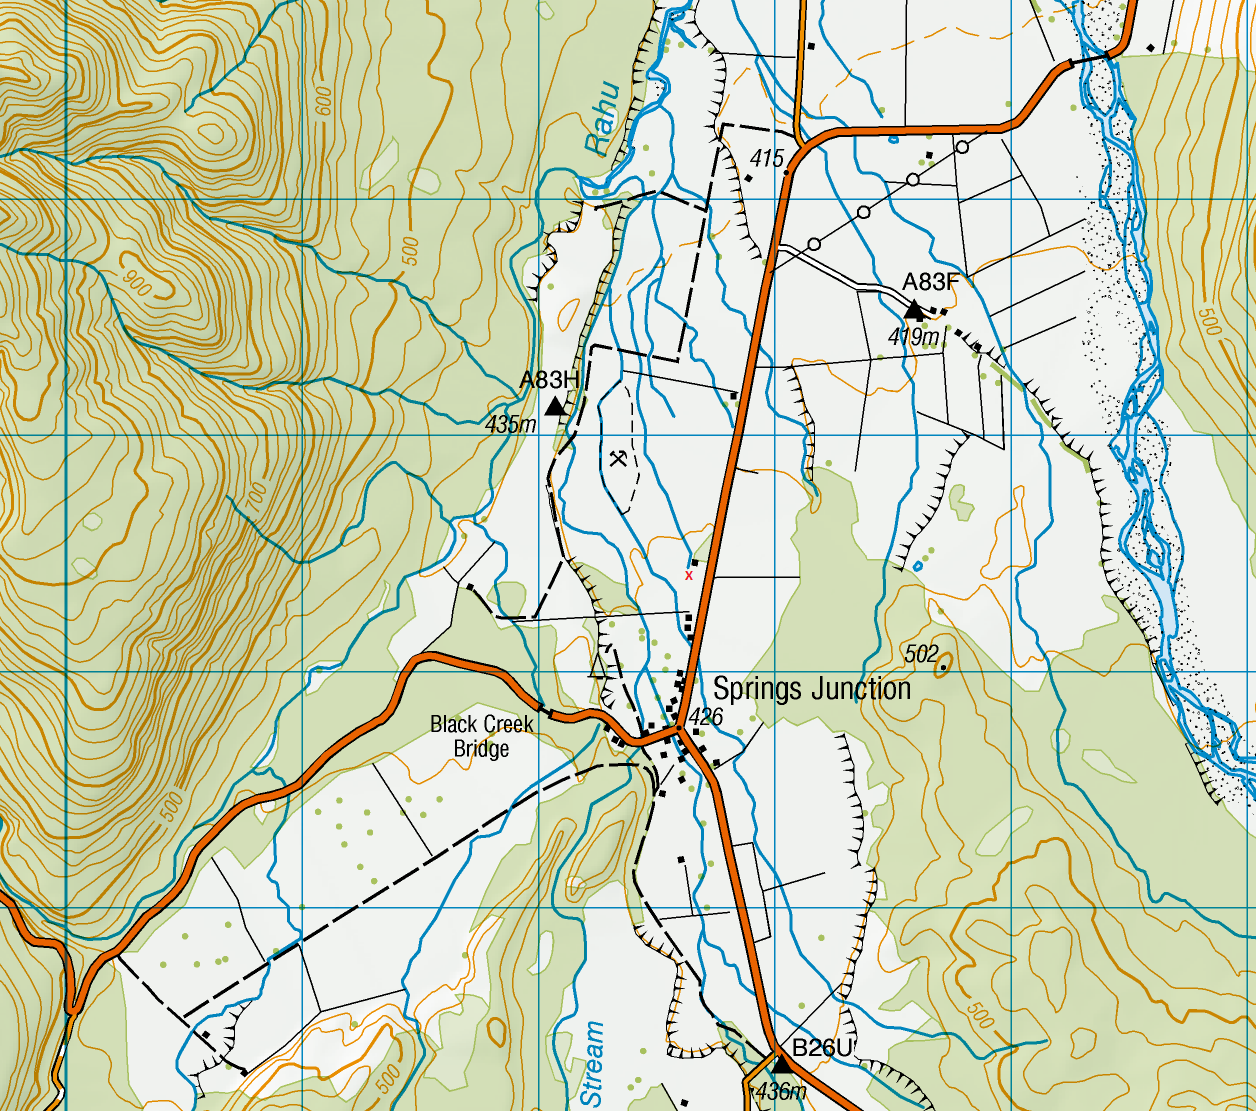
\includegraphics[width=5.5cm]{BachLocation}
\end{center} 
\end{minipage}
\hspace{.05\linewidth}
\begin{minipage}{.3\linewidth}
\begin{flushright} 
    \includegraphics[width=4.5cm]{BachInSnow}
\end{flushright} 
\end{minipage}
\end{figure}

\section{Directions}
  The house is on the west side of Highway 65 at the 60kph sign just to the north of Springs Junction.  It's \href{https://map.what3words.com}{what3words} address is \textit{\href{https://map.what3words.com/running.predominant.nicely}{running.predominant.nicely}}.  It is through the second gate on the right off ``Josie's Way''.  Currently it is the only building on the sub-division.

\section{Your stay}
\begin{itemize}
  \item Generally, we prefer to share meals with guests.  However, you are welcome to cook for yourself if you prefer.
  \item I am vegetarian and prefer that meat is not fried inside.
  \item The water in the taps comes from a well, but we also save rain-water for drinking.  Neither the well-water nor the rain-water have been tested or treated.
  \item The house is off-grid (i.e., powered entirely from the solar panels).  The system is deliberately marginal so that one has to be conscious of power usage.  The inverter is pure sine-wave and should be safe for electronic equipment.
  \item In winter the water is heated by the fire, but in summer we rely on the sun's energy.  Thus the `warm showers' may have to be brief.
  \item There is an outdoor bath which takes 1-1.5 hours to heat (if the cover is put on it).  There is a blue pseudo-sheepskin mat hanging up by the `Pyroclassic' fire to sit on when in the bath (the base of the bath can get quite hot).
  \item There is no rubbish or recycling service at Springs Junction, so please be prepared to take your non-compostable rubbish with you.
  \item We use a composting toilet, the Kiwi-Bog.  This is an exclusively sit-down facility (men may pee outside on the plants).  There are instructions on the shelf in the toilet: \textbf{please read these}.
  \item Compostable vegetable material can be put into the wooden compost bin by the bath.  Please don't put meat scraps in either the toilet or compost bin (bury them or take them with you).
  \item \textbf{No smoking} in the bach or on the decking.  If smoking outside, please do not litter (i.e., take the butts with you).
  \item Please fill-in the Visitor's Book.
\end{itemize}

\subsection{Hazards}
Care should be taken with the ladder to the sleeping loft (it is a ladder not stairs).

\bigskip
Peter Alspach\\paalspach@gmail.com\\(022) 528 7529

\end{document}
